%%%%%%%%%%%%%%%%%%%%%%%%%%%%%%%%%%%%%%%%%%%%%%%%%%%%%%%%%%%%%%%
% Set up document
%%%%%%%%%%%%%%%%%%%%%%%%%%%%%%%%%%%%%%%%%%%%%%%%%%%%%%%%%%%%%%%

\documentclass[xcolor={usenames,dvipsnames}]{beamer}
\usetheme{Madrid}
\setbeamersize{text margin left=5mm,text margin right=5mm}

% Dark background with non-white words: 
% \usecolortheme{owl}
% \setbeamercolor{normal text}{fg=yellow}
% \setbeamercolor{frametitle}{fg=yellow}
% \usebeamercolor[fg]{normal text}

% Used to create a section slide between section
\AtBeginSection[]{
  \begin{frame}[noframenumbering, plain]
  \vfill
  \centering
  \begin{beamercolorbox}[sep=8pt,center,shadow=true,rounded=true]{title}
    \usebeamerfont{title}\insertsectionhead\par%
  \end{beamercolorbox}
  \vfill
  \end{frame}
}

% Used to create a subsection slide between subsections
% \AtBeginSubsubsection{\frame{\subsubsectionpage}}
\AtBeginSubsection[]{
  \begin{frame}[noframenumbering, plain]
  \vfill
  \centering
  \begin{beamercolorbox}[sep=8pt,center,shadow=true,rounded=true]{title}
    \usebeamerfont{title}\insertsectionhead:\par\phantom{space please}\par\insertsubsectionhead\par%
  \end{beamercolorbox}
  \vfill
  \end{frame}
}


% Remove default navigation symbols and add just  page number
\setbeamertemplate{navigation symbols}{} % Clear default navigation
% \addtobeamertemplate{navigation symbols}{}{%
%     \usebeamerfont{footline}%
%     \usebeamercolor[fg]{footline}%
%     \hspace{1em}%
%     \insertframenumber/\inserttotalframenumber
% }

% Remove from footer the names, institution, date...
% and just leave page number:
\setbeamertemplate{footline}[frame number]


% For manual font size:
\usepackage{anyfontsize}

% For smaller URLs:
\newcommand{\smallurl}[1]{\textcolor{blue}{\fontsize{4pt}{4.8pt}\selectfont \url{#1}}}
%%%%%%%%%%%%%%%%%%%%%%%%%%%%%%%%%%%%%%%%%%%%%%%%%%%%%%%%%%%%%%%

% Title page

\title{Open science in the stroke projects}

\author{Anna Laws, Michael Allen, Kerry Pearn}

%\institute{Overleaf}
\date{November 2022}


\begin{document}

%\frame{\titlepage}

\begin{frame}
\titlepage

\end{frame}


\begin{frame}
\frametitle{Outline}
\tableofcontents
\end{frame}

%%%%%%%%%%%%%%%%%%%%%%%%%%%%%%%%%%%%%%%%%%%%%%%%%%%%%%%%%%%%%%%

\section{Stroke Projects}

\begin{frame}{The emergency stroke pathway}

\begin{center}
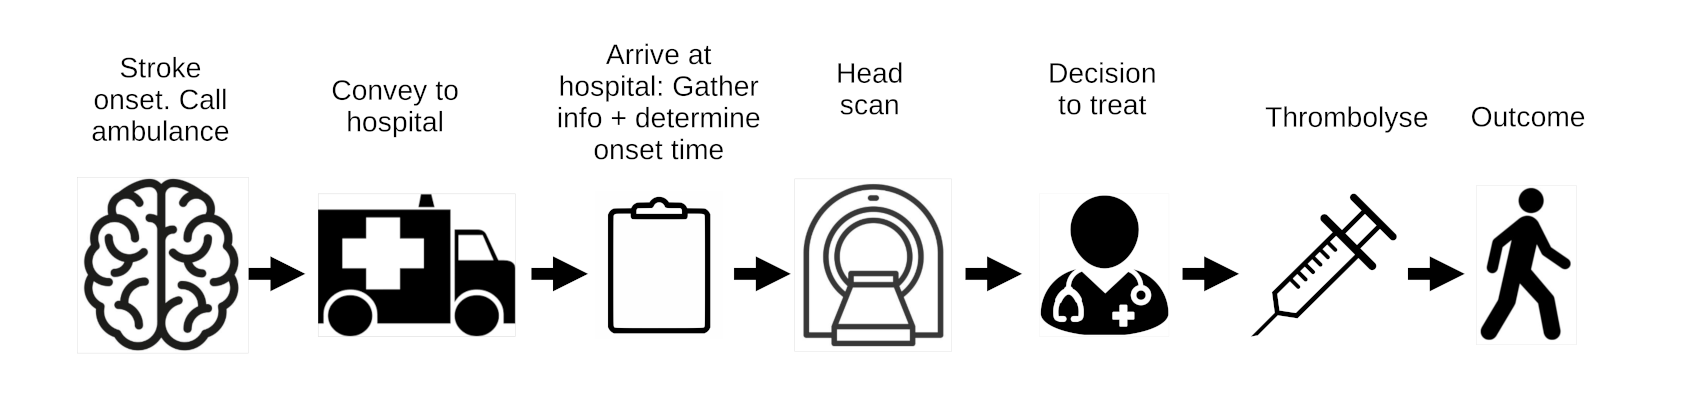
\includegraphics[width=0.99\textwidth]{./images/pathway}
\end{center}

\vspace{4mm}
The central problem we are investigating is that there is a NHS target to give clot-busting drugs (\emph{thrombolysis}) to 20\% of patients, but actually only 11\% patients are receiving them (and this varies from 5\% to 25\% between hospitals).

\end{frame}


%%%%%%%%%%%%%%%%%%%%%%%%%%%%%%%%%%%%%%%%%%%%%%%%%%%%%%%%%%%%%%%


\begin{frame}{Stroke projects}

\begin{itemize}
    \setlength\itemsep{2.5mm}
    \item SAMueL: Stroke Audit Machine Learning 
    \begin{itemize}
        \item Emergency stroke clinical pathway simulation
        \item Machine learning to learn and compare clinical decision-making between hospitals
        \item Detailed (disability-level) clinical outcome model
        \item Health economics model
    \end{itemize}
    \item OPTIMIST: OPTimising IMplementation of Ischaemic Stroke Thrombectomy
        \begin{itemize}
            \item Modelling and optimising the pre-hospital emergency stroke pathway.
        \end{itemize}
    \item Mobile Stroke Units (hopefully!)
    \item Geographic modelling (update)
    \item Whole stroke system modelling?
\end{itemize}
    
\end{frame}


%%%%%%%%%%%%%%%%%%%%%%%%%%%%%%%%%%%%%%%%%%%%%%%%%%%%%%%%%%%%%%%
\section{Open Science Tooling in Stroke Work}

\begin{frame}{Caveats}

\begin{itemize}
    \setlength\itemsep{2mm}
    \item Learning these tools takes time
    \item We are still learning
    \item We still shout at things at times
    \item Other tools exist
    \item These are probably \emph{not} tools for people who's job keeps them in Microsoft Office most of the day
\end{itemize}

\vspace{3mm}
But.....
\vspace{3mm}

\begin{itemize}
    \setlength\itemsep{2mm}
    \item It works
    \item We just use free/open tools
    \item The benefits, and quality of what may be produced, far outweigh the challenges
\end{itemize}

\end{frame}

%%%%%%%%%%%%%%%%%%%%%%%%%%%%%%%%%%%%%%%%%%%%%%%%%%%%%%%%%%%%%%%

\begin{frame}{Our stack of tools}


\begin{center}
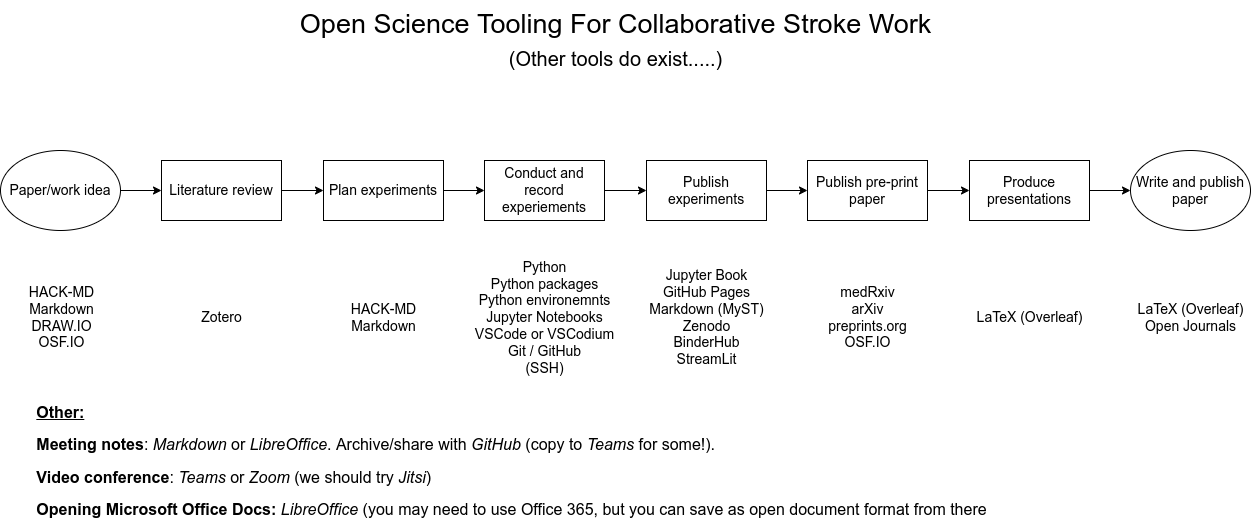
\includegraphics[width=0.99\textwidth]{./images/open_science_light}
\end{center}

\end{frame}

%%%%%%%%%%%%%%%%%%%%%%%%%%%%%%%%%%%%%%%%%%%%%%%%%%%%%%%%%%%%%%%

\begin{frame}{Examples of tools}

\footnotesize

\begin{itemize}
    \item Jupyter Book \& Notebooks: 
    \url{https://samuel-book.github.io/samuel_shap_paper_1/introduction/intro.html}
    \item GitHub: 
    \url{https://github.com/samuel-book/samuel_shap_paper_1}
    \item Zenodo: 
    \url{https://zenodo.org/account/settings/github/}
    \item VS Code
    \item Overleaf:
    \url{https://www.overleaf.com/project/636ba04103f728a89c7b5a5d}
    \item HackMD: 
    \url{https://hackmd.io/@N4jCROVmS9SqGmgj3U66XA/HJPwxmtSs}
    \item Zotero: 
    \url{https://www.zotero.org/groups/4707796/mja_stroke/items/H5JR5N99/library}
    \item Open Print Servers:
    \url{https://www.medrxiv.org/content/10.1101/2020.07.18.20156653v1}
    \item OSF (Open Science Framework):
    \url{https://osf.io/dashboard}
    \item Streamlit: 
    \url{https://samuel2-stroke-outcome.streamlit.app/Interactive_demo}
    \item BinderHub: 
    \url{https://github.com/MichaelAllen1966/2004_covid_dialysis}
    
    
\end{itemize}


\end{frame}

%%%%%%%%%%%%%%%%%%%%%%%%%%%%%%%%%%%%%%%%%%%%%%%%%%%%%%%%%%%%%%%

\begin{frame}{General lessons}

\begin{itemize}
    \setlength\itemsep{3mm}
    \item Open Science takes time - quality is not necessarily cheap
        \begin{itemize}
            \item We tend to go through, and refine, notebooks several times to check for errors, make them clear, clean, and understandable
        \end{itemize}
    \item Working with others helps
        \begin{itemize}
            \item We pass notebooks around at times - both for coding and summarising
            \item If a mistake gets through, no single person is to blame
            \item Psychological support
        \end{itemize}
    \item Git can be hard! Allow time to get used to it
    \begin{itemize}
            \item Create a branch for each notebook you work on
            \item Commit and push often
            \item Visual Studio Code has nice Git and GitHub integration (sorry Tom)
        \end{itemize}
    \item If you are new to \LaTeX, don't start with presentations (or posters)
\end{itemize}

\end{frame}

%%%%%%%%%%%%%%%%%%%%%%%%%%%%%%%%%%%%%%%%%%%%%%%%%%%%%%%%%%%%%%%
\section{The PenCHORD Way?}

\begin{frame}{The PenCHORD Way?}

\begin{itemize}
    \setlength\itemsep{3mm}
    \item Do we want a set of tools we more actively support and train people in?
    \item \emph{Supportive} not \emph{coercive}
    \item If so, what tools?
    \item What documentation/training material?
    \begin{itemize}
        \item Jupyter Book?
        \item Other?
    \end{itemize}
    \item How do we involve everyone in developing the PenCHORD Way?
\end{itemize}

\end{frame}

\end{document}


